\documentclass{scrartcl}

\usepackage{biblatex}
\bibliography{refs}

\usepackage{tikz-cd}

\usepackage{amssymb}
\usepackage{amsmath}
\usepackage{listings}

\lstset{ %
  basicstyle=\ttfamily,
  breaklines=true,
  captionpos=b,
  showspaces=false,
  showtabs=false,
  language=Haskell,
  escapechar=@,
  deletekeywords={Nothing,Just,False,True,putStrLn,fail,fromJust,lookup,Num,exp,free,snd,String,
  return,error,otherwise,not,show,read,Eval,Read,readsPrec,print,insert,length,id,try,Left,Right,union,
  join,Monad,Functor,Either,all,Maybe,mapM},
}

\usepackage{hyperref}
\newcommand{\lst}[1]{\lstinline!#1!}
\newcommand{\Cat}[1]{\mathbf{#1}}
\newcommand{\Op}[1]{#1^{\mathbf{op}}}
\newcommand{\Arr}[1]{#1^{\rightarrow}}
\newcommand{\iso}[0]{\cong}
\newcommand{\comma}[2]{#1 \downarrow #2}
\newcommand{\adjoint}[0]{\dashv}
\newcommand{\Hom}[3]{\mathit{Hom}_{#1}(#2,#3)}
\newcommand{\slice}[2]{#1 / #2}


\title{Category Theory Study Group}
\date{}

\begin{document}

\maketitle

\section*{Third Session}
For the third session, read 1.7 - 2.2.

\begin{enumerate}

\item
  Use the universal mapping property of the free monoid to construct a monoid homomorphism $M(\mathbb{N}) \rightarrow (\mathbb{N},+,0)$ and $M(\mathbb{N}) \rightarrow (\mathbb{N},\ast,1)$ for a function $f: \mathbb{N} \rightarrow \mathbb{N}$ defined by $f(x) = x \ast 4$. Apply this homomorphism to a few inputs to see what it does.

\item
  For the next exercise assume the following two datatypes,
  \begin{lstlisting}[gobble=4]
    data List a = Cons a (List a) | Nil
    data Tree a = Empty | Leaf a | Node (Tree a) (Tree a)
  \end{lstlisting}
  where \lst{Tree} is a higher inductive type, which means that it comes equipped with the equations
  \begin{align}
  &\forall\mathtt{t,\ Node\ t\ Empty\ =\ t} \\
  &\forall\mathtt{t,\ Node\ Empty\ t\ =\ t} \\
  &\forall\mathtt{t_1,t_2,t_3,\ Node\ t_1\ (Node\ t_2\ t_3)\ =\ Node\ (Node\ t_1\ t_2)\ t_3}.
  \end{align}
  
  Take a look at the Haskell module \lst{Data.Foldable}\footnote{Warning, there are some spoilers in the documentation at the top of the page. Use this link to avoid the spoilers: \url{https://hackage.haskell.org/package/base/docs/Data-Foldable.html\#v:fold}}.
  Is there a function that is similar to the unique mapping property of the free monoid?
  Implement this function as part of proving that \lst{List} and \lst{Tree} enjoy the property of the free monoid.
  Use proposition 1.10 to construct an isomorphism between \lst{List} and \lst{Tree} in the category $\Cat{Mon}$.

\clearpage
\item
  What are the free categories for the following graphs? Draw diagrams of these categories including identities.
  \begin{center}
  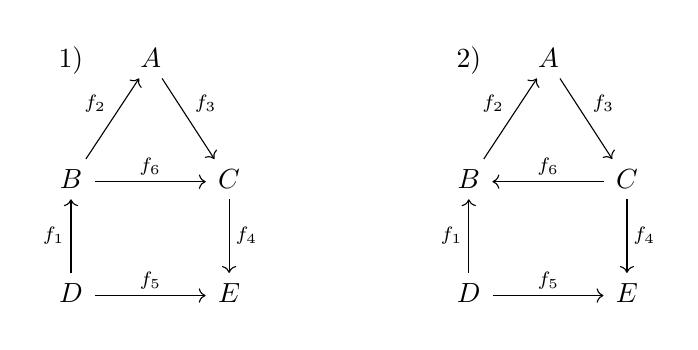
\begin{tikzpicture}
    \node(A){
    \begin{tikzcd}[row sep=large, column sep=small]
      1) & A \arrow[rd,"f_3"] & \\
      B \arrow[ru, "f_2"] \arrow[rr,"f_6"] & & C \arrow[d,"f_4"] \\
      D \arrow[rr,"f_5"] \arrow[u,"f_1"]  & & E
    \end{tikzcd}
    };
    \node[left of=A,xshift=40ex](B){
    \begin{tikzcd}[row sep=large, column sep=small]
      2) & A \arrow[rd,"f_3"] & \\
      B \arrow[ru, "f_2"] & & C \arrow[ll,"f_6" above] \arrow[d,"f_4"] \\
      D \arrow[rr,"f_5"] \arrow[u,"f_1"]  & & E
    \end{tikzcd}
    };
  \end{tikzpicture}
  \end{center}
  How many free categories on graphs are there which have exactly six arrows? Draw the graphs that generate these categories.

  Define a higher-inductive datatype for free categories.
  
\item
  What are (split) monoic and (split) epics in the category of matricies, monoids, graphs? Give at least two examples for each monics and epics.

\item Prove that two initial (terminal) objects are unique up to unique isomorphism.

\item What are initial (terminal) objects in $\Cat{Set}, \Cat{Cat}, \Cat{Graphs}, \Cat{Mon}, \slice{\Cat{Set}}{A}, \slice{A}{\Cat{Set}}$? What are arrows $1 \rightarrow X$, and $X \rightarrow 0$.
\end{enumerate}

% \printbibliography

\end{document}

%%% Local Variables:
%%% mode: latex
%%% TeX-master: t
%%% End:
